%!TEX root = main.tex

\documentclass[../main.tex]{subfiles}

\begin{document}

\chapter{Introduction}
\section{Motivation}
One of the more unique methods of playing guitar is an approach referred to as “slide guitar.” This consists of using a smooth rigid tube (the slide) to control the length of the string, instead of the frets and fingers. The slide rests on top of the string and does not touch the fingerboard or frets. In this way, it acts as a movable string termination and influences the vibration of the string by creating a new load termination in between the nut and the bridge \citetwo{evangelista_physical_2012}. This allows unique articulations and pitch inflections to be generated as the player is no longer constrained to the pitches provided by the fret locations. Vibrato is one of the characteristic articulations of slide playing. Figure~\ref{fig:acoustic_chrome} shows a player using a chrome slide on an acoustic guitar.

\begin{figure}[h]
    \centering
    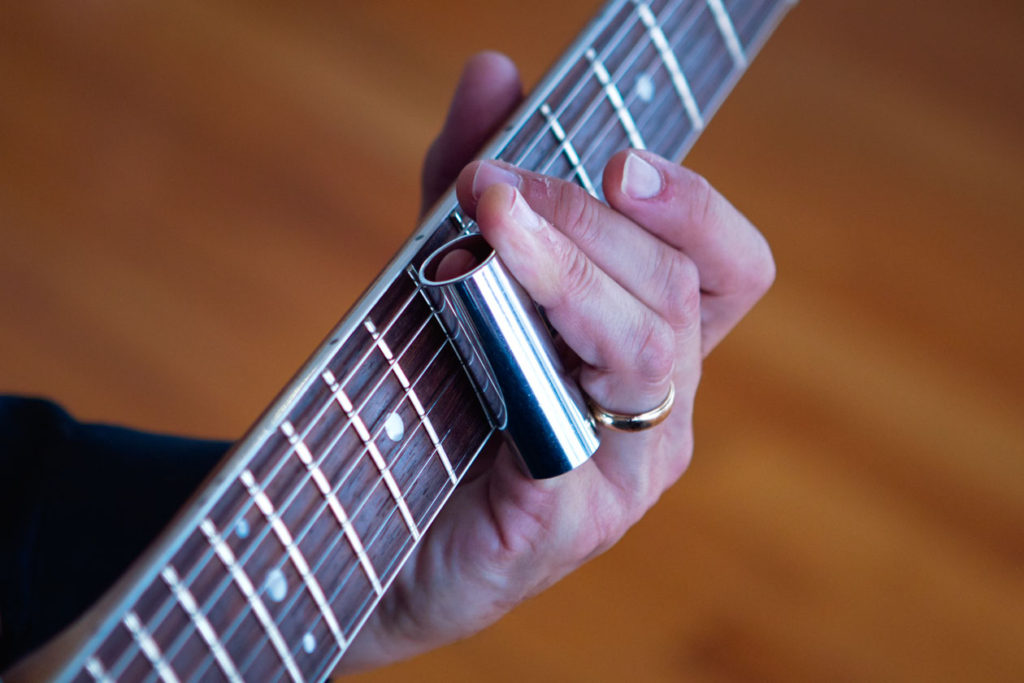
\includegraphics[scale=.30]{./images/pictures/Slide-guitar-1024x683.jpg}
    \caption{An acoustic guitar played with a chrome slide.}
    \label{fig:acoustic_chrome}
\end{figure}

Traditionally, slides are made from ceramic or metal \citetwo{bhanuprakash_finite_2020}. This results in a smooth/polished surface for the slide. The density of the material is important as this determines the slide's mass and correspondingly the force it applies to the string. Figure~\ref{fig:slide_types} illustrates different slides made out of a variety of materials. The slide's surface texture and mass are important as they influence how the slide interacts with the surface of the string. This interaction creates a new timbral component which is also influenced by the slide’s velocity \citetwo{pakarinen_virtual_2008}.

\begin{figure}[h]
    \centering
    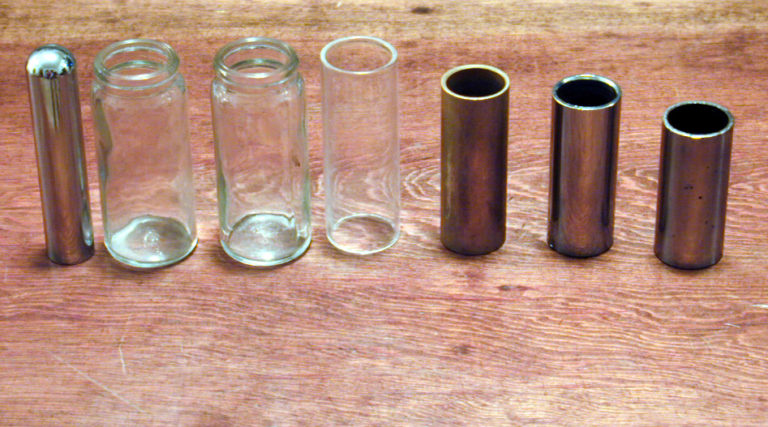
\includegraphics[scale=.35]{./images/pictures/Slide-guitar-different-slides-768x427.jpg}
    \caption{A selection of slides made from different materials, all of which are comparatively smooth.}
    \label{fig:slide_types}
\end{figure}

In the case of wound strings, two new sounds are created. The first is a time-varying harmonic component due to the interaction of the slide with the spatially periodic pattern of windings on the string’s surface (inherent in a wound string’s construction) \citetwo{pakarinen_analysis_2007}. The second component is due to the stimulation of the string’s longitudinal modes as the slide introduces disturbances in this direction when it impacts the ridges of the windings. As the slide does not provide sufficient force to change the longitudinal length, the longitudinal mode frequencies are static, regardless of the motion of the slide \citetwo{pakarinen_analysis_2007}. Figure~\ref{fig:slide_string_zoom} shows a close-up illustration of a slide interacting with a wound string.

\begin{figure}[h]
    \centering
    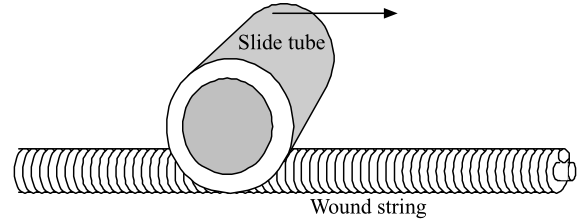
\includegraphics[scale=1]{./images/pictures/slide_wound_string_zoom.PNG}
    \caption{A close-up illustration of a slide on wound string \citetwo{pakarinen_virtual_2008}.}
    \label{fig:slide_string_zoom}
\end{figure}

Unwound strings have a uniform surface, lacking the ridges created by windings which a slide impacts while traveling the length of the string. Correspondingly, the coefficient of friction between the unwound string and slide is comparatively much lower than in the wound-string case. This drastically reduces the coupling between the slide and the unwound string from a longitudinal standpoint, with the result that the longitudinal modes are not audible. As a result, the contact sound generated for unwound strings is more akin to white-noise whose amplitude is scaled by the slide velocity and lacks a harmonic component \citetwo{pakarinen_virtual_2008}. 

The original sound synthesis model which serves as the impetus for this thesis comes from \citetwo{pakarinen_virtual_2008}. The goal of this project is to explore this model more fully from a digital signal processing standpoint as compared to the description in the aforementioned paper. This includes aspects related to its implementation, verification and inherent limitations. Possible refinements to the physical modeling will be investigated as well as aspects related to parametrizing the control signals to generate usable and interesting musical signals. The implementation is done in MATLAB to facilitate easier analysis and verification of the model.

This model was mainly chosen due to a match between its complexity and the author's skills at the outset of the thesis. The paper is the only one which emphasized real-time implementations and that was a potential outcome when the thesis commenced. The initial descriptions also contain physical measurements as part of the model's development, which the author had an interest in recreating. Additionally, the details of the implementation are readily available as PD patches in Appendix B of \citetwo{puputti_real-time_2010}.

\section{Thesis Organization}
The thesis is organized into seven different chapters as described below.

\subsubsection{Chapter 1 - Introduction}
This chapter provides a brief overview of the slide guitar, what the thesis hopes to achieve as well as how the thesis is organized.

\subsubsection{Chapter 2 - Background}
Chapter 2 will  elaborate upon the necessary theoretical knowledge to understand the rest of the thesis. It is not meant to be exhaustive as both digital signal processing and physical modeling are large and broad fields themselves. The aim is to introduce as much theory as is necessary as well as provide references if an interested reader wishes to find more details. Other approaches and techniques will be examined as well.

\subsubsection{Chapter 3 - Description of Slide Guitar Synthesis Model}
After the necessary theory has been introduced, the architecture of the slide guitar synthesizer will be described as well as its constituent components. Some aspects will have already been introduced in the background, however more details will be provided to fully elucidate the mechanics of the model.

\subsubsection{Chapter 4 - Verification Of Slide Model and Constituent Components}
The techniques used to verify the correctness of the model will be discussed as well as any limitations inherent to it. Audio examples will be provided to help develop an aural intuition for the sounds. However, the synthesis parameters will often not be realistic and physically informed as their goal is to illustrate algorithmic correctness of the model as opposed to usable sonic potential (which will be covered in Chapter 6).

\subsubsection{Chapter 5 - Physical Measurements of Slide Sounds}
In this section, the physical experiments which were performed during the development of this model will be described. As will be shown in both Chapters 2 \& 3, there is a strong physical basis for the synthesizer model. Many of the model's parameters have a physical correlate, hence why this section comes after the model's description. Some of the experiments will be recreating work from the original paper, while others will attempt to refine the model to make it more physically informed.

\subsubsection{Chapter 6 - Sound Design and Control Signals}
After the model has been described and verified (both algorithmically and physically), the next step is to tune the parameters and control signals. This chapter aims to explore how the parameters were tuned as well as the different architectural and component decisions which were explored in an attempt to create the ``best" sounding synthesizer. It will also examine strategies related to generating control signals to achieve different sounds.

\subsubsection{Chapter 7 - Conclusion and Future Work}
The last section provides a brief summary of what has been explored in the thesis as well as expounds upon opportunities for improvement and future research.

\end{document}